\section{Resultados}\label{resultados}

\subsection{Caracterização do alvo e dos
dados}\label{caracterizauxe7uxe3o-do-alvo-e-dos-dados}

Esta seção apresenta os resultados consolidados do estudo para a
disciplina. O benchmark comparativo foi realizado por validação cruzada
agrupada e a avaliação externa foi executada uma vez após o congelamento
dos candidatos na visão \texttt{repository-only}. Os resultados das
visões textuais são apresentados em análises separadas.

Entre as skills reutilizadas, \texttt{repository\_count} apresenta
distribuição fortemente assimétrica e sobredispersa. A média é 5,075
repositórios, a mediana é 2, a variância é 112,22 e a razão entre
variância e média é 22,11. O maior valor observado no conjunto de
desenvolvimento é 390 repositórios. A diferença entre média e mediana
indica que poucas skills concentram valores muito elevados.

Os quantis do desenvolvimento, calculados somente nas 25.918 skills
reutilizadas, são:

\begin{longtable}[]{@{}lrrrrr@{}}
\toprule\noalign{}
Quantil & P50 & P75 & P90 & P95 & P99 \\
\midrule\noalign{}
\endhead
\bottomrule\noalign{}
\endlastfoot
Repositórios & 2 & 4 & 8 & 16 & 55 \\
\end{longtable}

A figura abaixo mostra a concentração nos valores baixos e a cauda
longa. No teste, o maior valor observado é 573. A transformação
\texttt{log1p} estabiliza o ajuste, mas o resultado agregado deve ser
lido junto com o erro na cauda.

\begin{figure}[!htbp]
\centering
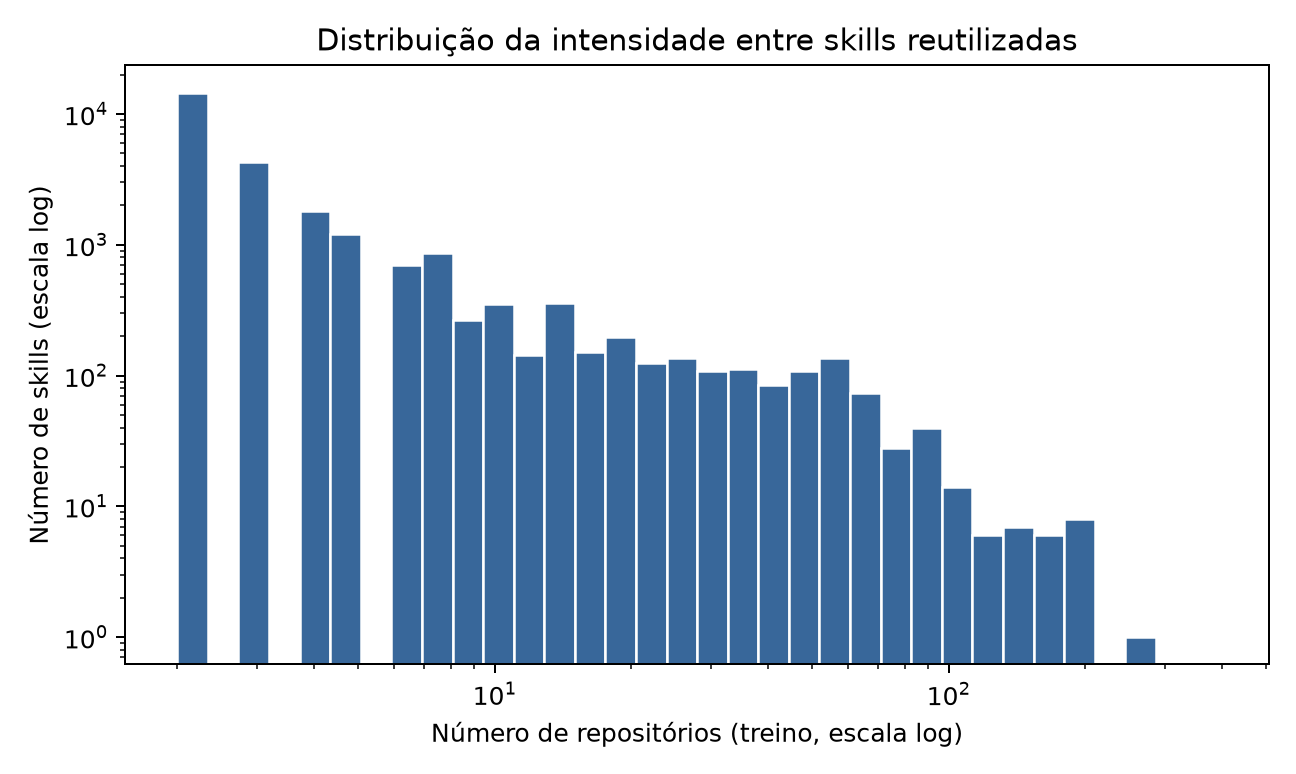
\includegraphics[width=0.88\linewidth]{figures/report_target_distribution.png}
\caption{Distribuição do alvo no desenvolvimento}
\label{fig:report-1}
\end{figure}

Nos atributos de repositório do desenvolvimento, \texttt{commit\_count}
está ausente em 69,86\% das 25.918 observações; estrelas, forks,
linguagem, licença e estado de fork têm aproximadamente 0,035\% de
ausência cada. \texttt{history\_fetched} e
\texttt{repo\_metadata\_fetched} não têm valores ausentes, mas sinalizam
a cobertura da coleta. A imputação e os indicadores de ausência foram
ajustados dentro de cada dobra. A tabela auditável está em
\texttt{repository\_missingness.csv}.

\subsection{Comparação das
representações}\label{comparauxe7uxe3o-das-representauxe7uxf5es}

A confirmação completa da configuração textual atual foi realizada com
10.000 candidatos TF-IDF e 500 termos selecionados, utilizando regressão
Ridge sobre \texttt{log1p(repository\_count)} e três dobras agrupadas. A
representação híbrida apresentou o menor RMSLE entre as três visões
avaliadas, embora a diferença para \emph{skill-only} seja pequena.

\begin{longtable}[]{@{}
  >{\raggedright\arraybackslash}p{(\linewidth - 6\tabcolsep) * \real{0.2000}}
  >{\raggedleft\arraybackslash}p{(\linewidth - 6\tabcolsep) * \real{0.2667}}
  >{\raggedleft\arraybackslash}p{(\linewidth - 6\tabcolsep) * \real{0.2667}}
  >{\raggedleft\arraybackslash}p{(\linewidth - 6\tabcolsep) * \real{0.2667}}@{}}
\toprule\noalign{}
\begin{minipage}[b]{\linewidth}\raggedright
Representação com Ridge
\end{minipage} & \begin{minipage}[b]{\linewidth}\raggedleft
RMSLE médio ± DP
\end{minipage} & \begin{minipage}[b]{\linewidth}\raggedleft
MAE médio
\end{minipage} & \begin{minipage}[b]{\linewidth}\raggedleft
Spearman médio
\end{minipage} \\
\midrule\noalign{}
\endhead
\bottomrule\noalign{}
\endlastfoot
\texttt{hybrid} & \textbf{0,568 ± 0,028} & 3,320 & 0,245 \\
\texttt{skill-only} & 0,572 ± 0,031 & 3,325 & 0,213 \\
\texttt{repository-only} & 0,588 ± 0,006 & 3,341 & 0,259 \\
\end{longtable}

Os resultados sugerem sinal nos atributos textuais e estruturais da
skill. A diferença média entre \texttt{hybrid} e \texttt{skill-only} é
de apenas 0,004 no RMSLE, menor que a variação entre dobras; não se pode
afirmar uma superioridade robusta do híbrido. \texttt{repository-only}
apresenta a maior correlação de Spearman nessa comparação, apesar do
pior RMSLE. Essas são estimativas de validação interna do Ridge; nenhum
dos dois modelos textuais foi avaliado no teste externo.

Essa diferença também reforça a necessidade de interpretar o modelo
híbrido com cautela. Parte do sinal pode estar associada ao contexto do
repositório, e não a propriedades intrínsecas da skill. Assim, a
vantagem híbrida não deve ser descrita como evidência de que o conteúdo
da skill, isoladamente, determina maior reutilização.

\subsection{Comparação das famílias de
modelos}\label{comparauxe7uxe3o-das-famuxedlias-de-modelos}

Como parte do trabalho da disciplina, foi executado um benchmark
completo com 25.918 observações, três dobras agrupadas e a representação
\texttt{repository-only}. Essa execução permite comparar todos os
regressores sobre a mesma matriz de atributos, sem o gargalo da
vetorização textual. Os resultados foram:

\begin{longtable}[]{@{}
  >{\raggedright\arraybackslash}p{(\linewidth - 6\tabcolsep) * \real{0.2000}}
  >{\raggedleft\arraybackslash}p{(\linewidth - 6\tabcolsep) * \real{0.2667}}
  >{\raggedleft\arraybackslash}p{(\linewidth - 6\tabcolsep) * \real{0.2667}}
  >{\raggedleft\arraybackslash}p{(\linewidth - 6\tabcolsep) * \real{0.2667}}@{}}
\toprule\noalign{}
\begin{minipage}[b]{\linewidth}\raggedright
Modelo \texttt{repository-only}
\end{minipage} & \begin{minipage}[b]{\linewidth}\raggedleft
RMSLE médio ± DP
\end{minipage} & \begin{minipage}[b]{\linewidth}\raggedleft
MAE médio ± DP
\end{minipage} & \begin{minipage}[b]{\linewidth}\raggedleft
Spearman médio
\end{minipage} \\
\midrule\noalign{}
\endhead
\bottomrule\noalign{}
\endlastfoot
Random Forest & \textbf{0,575 ± 0,008} & 3,282 ± 0,120 & 0,287 \\
HistGradientBoosting & 0,583 ± 0,019 & 3,312 ± 0,034 & 0,255 \\
Gradient Boosting & 0,587 ± 0,010 & \textbf{3,173 ± 0,129} &
\textbf{0,317} \\
Ridge & 0,588 ± 0,006 & 3,341 ± 0,156 & 0,259 \\
Decision Tree & 0,593 ± 0,017 & 3,321 ± 0,073 & 0,282 \\
KNN & 0,610 ± 0,027 & 3,452 ± 0,054 & 0,214 \\
\end{longtable}

O Random Forest apresentou o menor RMSLE, enquanto o Gradient Boosting
obteve o menor MAE e a maior correlação de Spearman. Isso mostra que a
escolha do melhor modelo depende do critério: o primeiro favorece erro
relativo na escala logarítmica, enquanto o segundo produz melhor erro
absoluto e ordenação. O resultado também confirma que a árvore isolada e
o KNN não oferecem vantagem consistente nessa representação.

Um spot-check agrupado comparou variantes dos dois candidatos. O Random
Forest com \texttt{max\_depth=12}, 100 árvores e
\texttt{min\_samples\_leaf=3} teve RMSLE de \textbf{0,575 ± 0,008},
contra 0,576 ± 0,008 com 200 árvores e 0,578 ± 0,004 com profundidade 8.
O Gradient Boosting com 200 estimadores e taxa 0,05 obteve \textbf{0,584
± 0,008}, ante 0,587 ± 0,010 com 100 estimadores. O critério de escolha
principal foi o RMSLE médio da validação agrupada.

O benchmark completo confirma que modelos ensemble não lineares capturam
relações úteis na visão \texttt{repository-only}, mas não há um vencedor
absoluto em todas as métricas. O desempenho de modelos mais flexíveis
deve ser interpretado junto com o risco de memorizar padrões
contextuais.

Após o congelamento da comparação da disciplina, os dois candidatos
selecionados foram treinados em todas as 25.918 observações de
desenvolvimento e avaliados uma única vez nas 6.479 skills reutilizadas
do teste externo. A sobreposição de \texttt{representative\_repo\_id}
foi zero.

\begin{longtable}[]{@{}lrrrr@{}}
\toprule\noalign{}
Modelo & RMSLE & MAE & MAE log1p & Spearman \\
\midrule\noalign{}
\endhead
\bottomrule\noalign{}
\endlastfoot
Random Forest & \textbf{0,5833} & 3,2663 & 0,4063 & \textbf{0,3667} \\
Gradient Boosting & 0,5907 & \textbf{3,1820} & \textbf{0,3903} &
0,2315 \\
\end{longtable}

O Random Forest já era o candidato principal pelo RMSLE da validação. Os
resultados externos estimam o desempenho dos dois candidatos na partição
reservada; o teste não redefiniu a escolha. Em comparação com a
referência constante que prediz a mediana do desenvolvimento (2
repositórios), o Random Forest reduz o RMSLE de \textbf{0,7142} para
\textbf{0,5833}, mas aumenta o MAE de \textbf{3,0665} para
\textbf{3,2663} e o MAE log1p de 0,3593 para 0,4063. A referência é
forte nas métricas médias porque a maior parte do teste tem contagem
baixa; o modelo melhora a diferenciação das contagens em RMSLE e
Spearman, mas não domina todos os critérios.

\subsection{Análise de erros por intensidade de
reutilização}\label{anuxe1lise-de-erros-por-intensidade-de-reutilizauxe7uxe3o}

Para o Random Forest \texttt{repository-only}, as faixas foram definidas
pelos quantis do desenvolvimento antes da auditoria das previsões
externas salvas. O erro cresce rapidamente acima de oito repositórios:

\begin{longtable}[]{@{}
  >{\raggedright\arraybackslash}p{(\linewidth - 10\tabcolsep) * \real{0.1304}}
  >{\raggedleft\arraybackslash}p{(\linewidth - 10\tabcolsep) * \real{0.1739}}
  >{\raggedleft\arraybackslash}p{(\linewidth - 10\tabcolsep) * \real{0.1739}}
  >{\raggedleft\arraybackslash}p{(\linewidth - 10\tabcolsep) * \real{0.1739}}
  >{\raggedleft\arraybackslash}p{(\linewidth - 10\tabcolsep) * \real{0.1739}}
  >{\raggedleft\arraybackslash}p{(\linewidth - 10\tabcolsep) * \real{0.1739}}@{}}
\toprule\noalign{}
\begin{minipage}[b]{\linewidth}\raggedright
Faixa observada no teste
\end{minipage} & \begin{minipage}[b]{\linewidth}\raggedleft
n
\end{minipage} & \begin{minipage}[b]{\linewidth}\raggedleft
RMSLE
\end{minipage} & \begin{minipage}[b]{\linewidth}\raggedleft
MAE
\end{minipage} & \begin{minipage}[b]{\linewidth}\raggedleft
Erro mediano (previsto − real)
\end{minipage} & \begin{minipage}[b]{\linewidth}\raggedleft
Subestimação
\end{minipage} \\
\midrule\noalign{}
\endhead
\bottomrule\noalign{}
\endlastfoot
≤2 (P50) & 3.648 & 0,395 & 1,33 & +1,12 & 0\% \\
3--4 (P50--P75) & 1.522 & 0,224 & 0,79 & +0,14 & 41,3\% \\
5--8 (P75--P90) & 683 & 0,428 & 2,22 & −2,11 & 90,2\% \\
9--16 (P90--P95) & 302 & 0,925 & 7,29 & −7,02 & 100\% \\
\textgreater16 (\textgreater P95) & 324 & 1,904 & 35,15 & −22,73 &
100\% \\
\end{longtable}

Acima do P95, a mediana observada é 27,5 e a mediana prevista é 4,45. Em
todo o teste, a maior previsão foi 10,29, frente à maior contagem
observada de 573. As figuras mostram a compressão das previsões e o
aumento do erro absoluto na cauda.

\begin{figure}[!htbp]
\centering
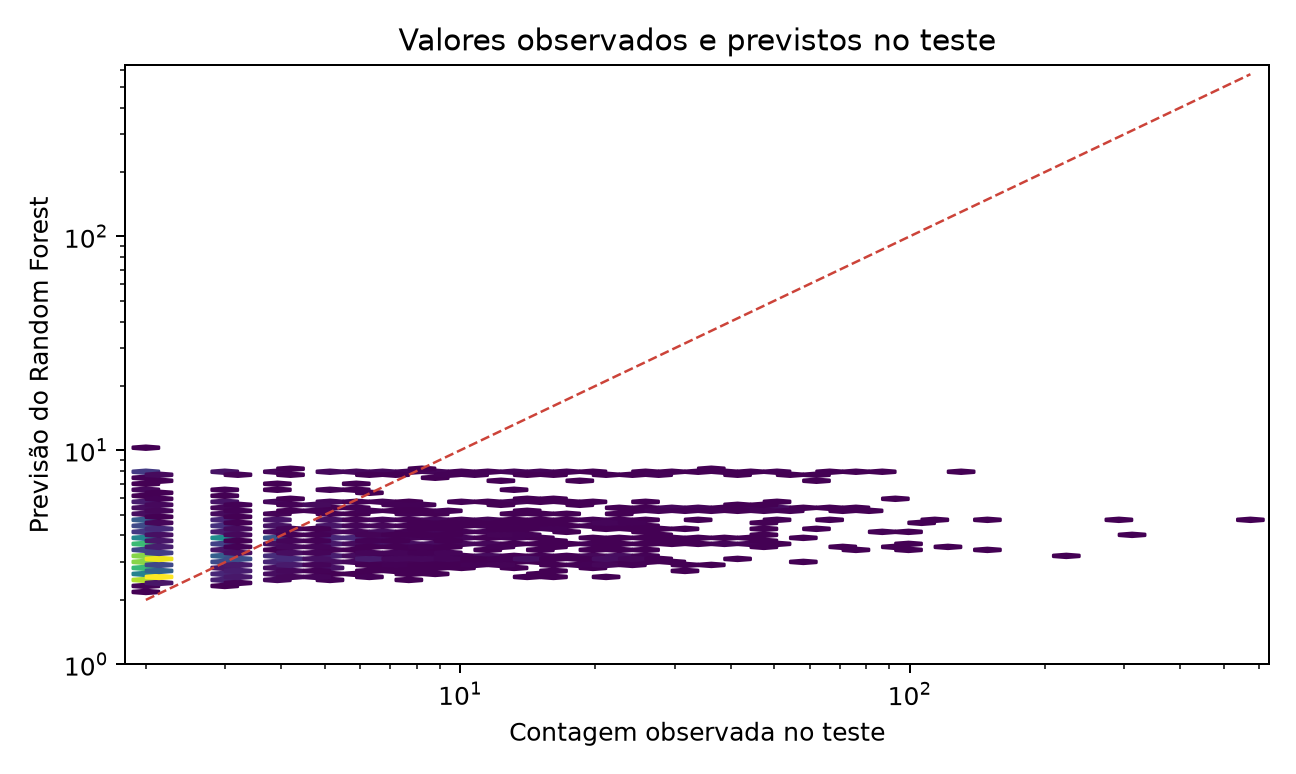
\includegraphics[width=0.88\linewidth]{figures/report_observed_vs_predicted.png}
\caption{Observado versus previsto no teste externo do Random Forest}
\label{fig:report-2}
\end{figure}

\begin{figure}[!htbp]
\centering
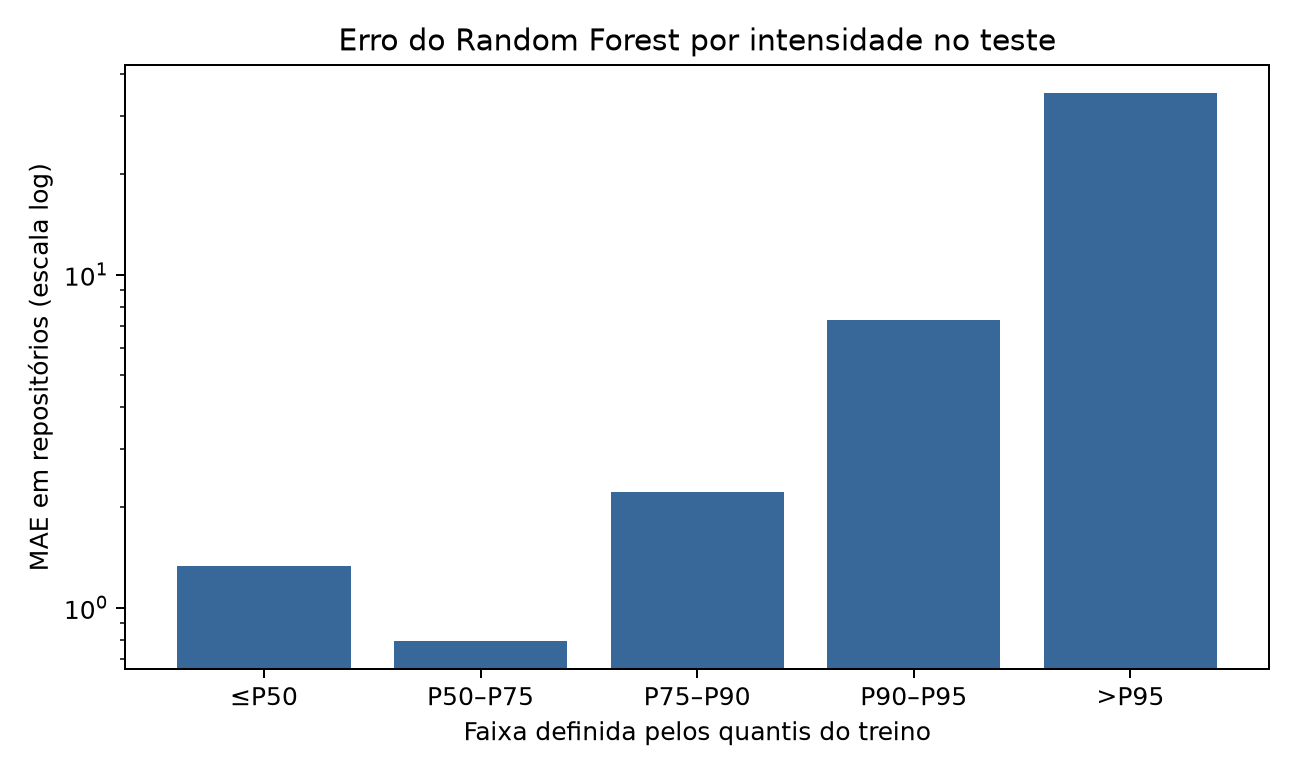
\includegraphics[width=0.88\linewidth]{figures/report_error_by_intensity.png}
\caption{MAE do Random Forest por faixa do alvo}
\label{fig:report-3}
\end{figure}

Como análise separada, a auditoria por quantis do Ridge híbrido na
validação encontrou subestimação crescente. Seus limiares foram
calculados no treino de cada dobra e aplicados à validação; não se trata
do teste do Random Forest.

\begin{longtable}[]{@{}lrrrr@{}}
\toprule\noalign{}
Faixa do alvo & Observações & RMSLE & MAE & Subestimação \\
\midrule\noalign{}
\endhead
\bottomrule\noalign{}
\endlastfoot
Até P50 & 14.593 & 0,432 & 1,46 & 6,7\% \\
P50--P75 & 6.087 & 0,302 & 1,11 & 48,3\% \\
P75--P90 & 2.773 & 0,466 & 2,25 & 89,7\% \\
P90--P95 & 1.232 & 0,890 & 7,20 & 99,7\% \\
Acima de P95 & 1.233 & 1,692 & 34,75 & 100,0\% \\
\end{longtable}

O modelo apresenta desempenho relativamente bom para a região central,
mas subestima de forma crescente os valores mais altos. Para as
observações acima do P95, a mediana do alvo é 33 repositórios, enquanto
a mediana da previsão é aproximadamente 6,22. Portanto, o RMSLE global
de 0,568 oculta uma falha importante para o subgrupo mais reutilizado.

Essa auditoria confirma que o Ridge híbrido também não representa
adequadamente a disseminação extrema. Os dois resultados de cauda
pertencem a modelos, representações e conjuntos de avaliação diferentes
e não são uma comparação direta.

\subsection{Robustez textual}\label{robustez-textual}

Foi comparado o texto bruto com uma versão que remove datas, números,
URLs e identificadores longos. A remoção desses artefatos alterou pouco
o desempenho: no modelo híbrido, o RMSLE passou de 0,568 para 0,570; no
modelo \texttt{skill-only}, passou de 0,572 para 0,575.

Essa pequena diferença sugere que os artefatos textuais identificados
não explicam sozinhos o sinal preditivo global. Entretanto, a análise
não permite concluir que todos os termos sejam semanticamente
relevantes. A representação textual ainda pode capturar convenções
editoriais, templates e padrões de distribuição associados às skills
reutilizadas.

\subsection{Explicabilidade e
consistência}\label{explicabilidade-e-consistuxeancia}

A análise global inicial do modelo híbrido encontrou sete dos 500 termos
selecionados com aparência de datas ou números; não foram identificados
URLs ou identificadores longos entre os principais termos. Alguns termos
recorrentes estavam relacionados a fragmentos editoriais, como
\texttt{date\_added} e \texttt{source\ community}, além de palavras de
conteúdo geral.

A auditoria de estabilidade em três dobras encontrou recorrência de
termos editoriais e de convenções de documentação. A versão com
artefatos mascarados reduziu os sinais explicitamente numéricos, mas não
eliminou termos associados a padrões editoriais. Esses achados devem ser
tratados como associações descritivas: a presença de um termo pode
indicar um template, uma origem comum ou um processo de publicação, e
não necessariamente uma propriedade que cause reutilização.

Na importância por impureza do Random Forest ajustado em todo o
desenvolvimento, os maiores valores pertencem a \texttt{repo\_stars}
(0,170), \texttt{history\_fetched} (0,153), indicador de ausência de
\texttt{commit\_count} (0,132) e \texttt{repo\_forks} (0,129). Essa
medida pode favorecer atributos com mais valores ou categorias. A
permutação dos oito atributos brutos na validação agrupada do
desenvolvimento fornece um contraste: aumento médio de RMSLE de 0,029 ±
0,013 para \texttt{repo\_language}, 0,014 ± 0,006 para
\texttt{commit\_count}, 0,013 ± 0,003 para \texttt{history\_fetched} e
0,012 ± 0,012 para \texttt{repo\_stars}. Uma das três dobras deu aumento
de apenas 0,0005 para estrelas, indicando instabilidade desse sinal. Foi
feita uma permutação por atributo e dobra, portanto a incerteza dessa
estimativa é limitada.

\begin{figure}[!htbp]
\centering
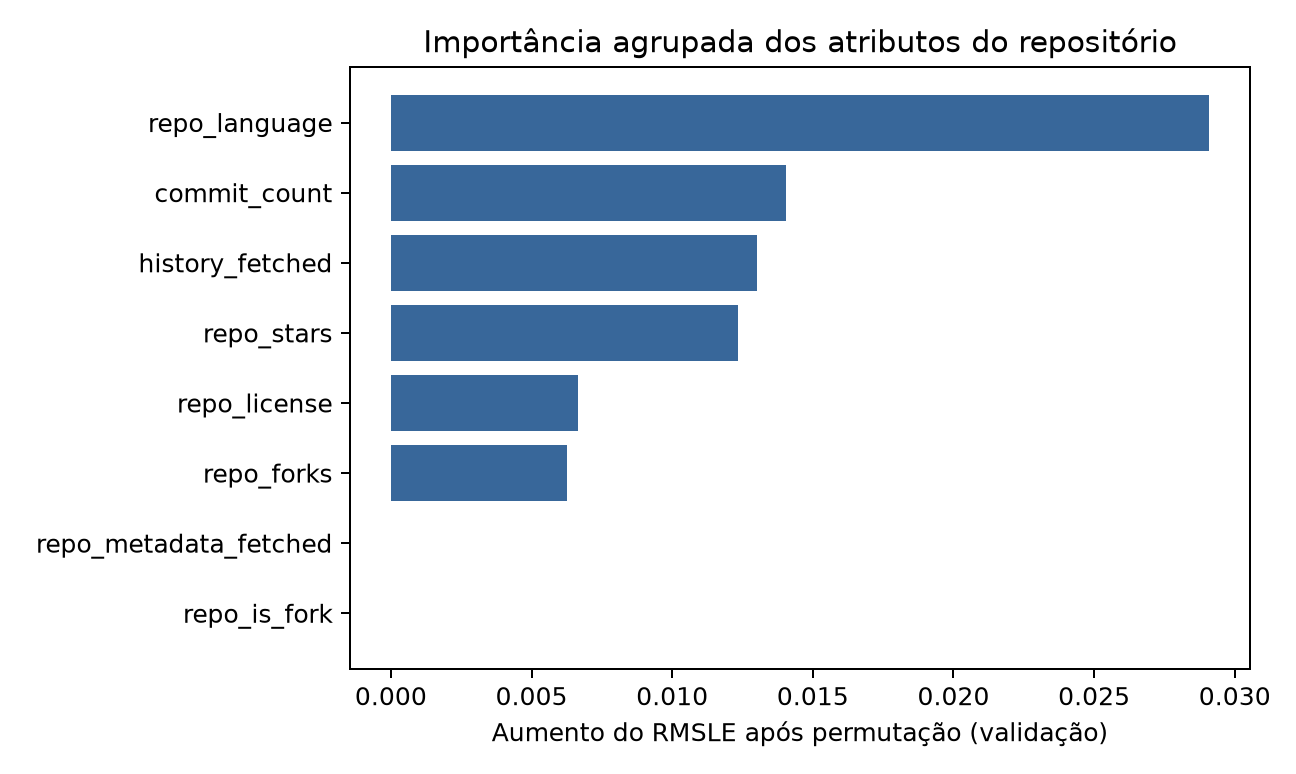
\includegraphics[width=0.88\linewidth]{figures/report_permutation_importance.png}
\caption{Aumento de RMSLE após permutação em validação agrupada}
\label{fig:report-4}
\end{figure}

Um cenário descritivo na primeira dobra variou \texttt{repo\_stars} para
0, 1, 3, 10, 100 e 1.000 em 1.000 observações de validação, mantendo as
outras entradas: a previsão média resultante foi 3,58; 3,62; 3,12; 3,29;
3,22; 3,17 repositórios. A resposta não é monotônica e alguns cenários
podem combinar valores incomuns de estrelas e forks. Logo, o experimento
não sustenta a afirmação de que aumentar estrelas causaria mais
reutilização. Toda essa explicação descreve o contexto do repositório,
não propriedades intrínsecas da skill.

\begin{figure}[!htbp]
\centering
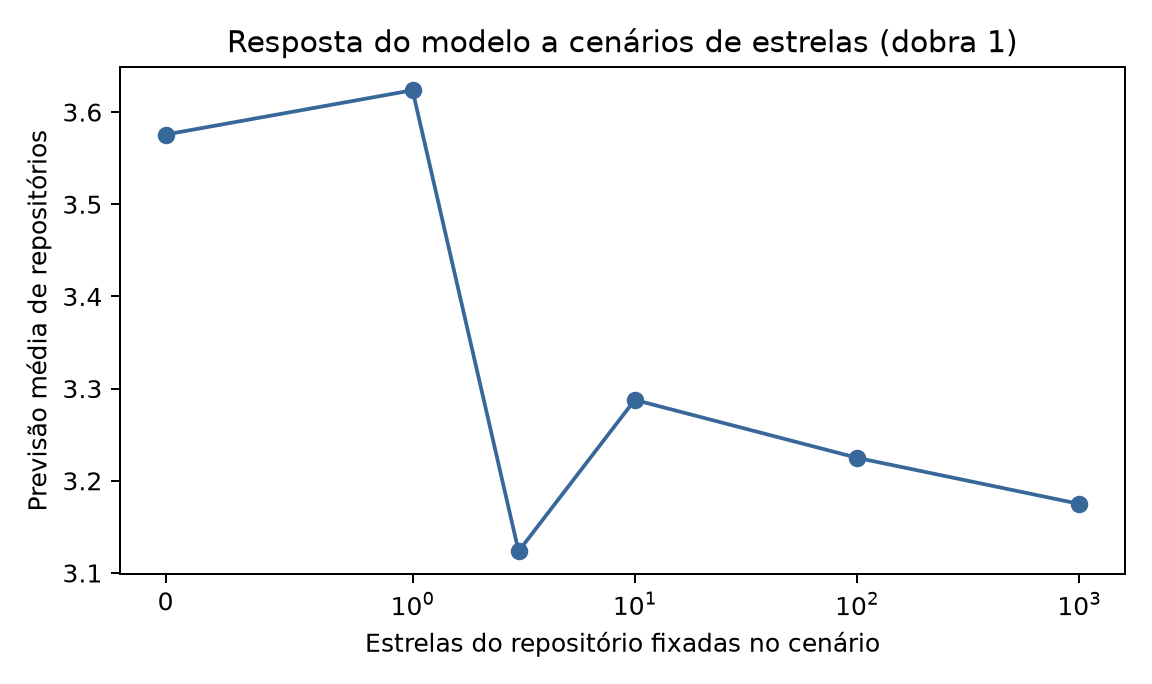
\includegraphics[width=0.88\linewidth]{figures/report_stars_scenario_fold1.png}
\caption{Previsão média ao variar estrelas no primeiro fold}
\label{fig:report-5}
\end{figure}

\subsection{Síntese dos resultados e estado da
avaliação}\label{suxedntese-dos-resultados-e-estado-da-avaliauxe7uxe3o}

Os resultados da disciplina sustentam quatro conclusões. Primeiro,
existe sinal preditivo mensurável para a intensidade de reutilização,
sobretudo na região central da distribuição. Segundo, a representação
híbrida apresenta pequena vantagem global no Ridge, mas a comparação
completa dos modelos foi realizada de forma controlada na visão
\texttt{repository-only}. Terceiro, a cauda de alta reutilização
continua sendo um problema relevante, com subestimação sistemática dos
maiores valores. Quarto, as explicações identificam padrões textuais e
contextuais plausíveis, mas não fornecem evidência de causalidade ou de
qualidade intrínseca das skills.

O Random Forest foi escolhido na validação pelo menor RMSLE médio e
obteve 0,5833 no teste externo. O Gradient Boosting apresentou MAE
externo menor (3,1820). Ambos os resultados são descritivos para a
divisão congelada. A referência constante superar o Random Forest em MAE
e a subestimação integral acima do P95 impedem uma conclusão de bom
desempenho geral. A análise de atributos da skill permanece parcial,
pois a comparação com texto foi interna e restrita ao Ridge.
